\documentclass[10pt]{article}

\title{ITF31519 - Assignment 2}
\author{Tobias Hallingstad}

\usepackage[utf8]{inputenc}
\usepackage[english]{babel}
\usepackage{minted}

\usepackage{graphicx}
\graphicspath{ {./images/} }

\begin{document}
    \begin{titlepage}
        \maketitle
    \end{titlepage}

    \newminted{python}{
        gobble=2,
        linenos
    }

    \section{Default values}
    I am basing the \texttt{MLPClassifier} on some default values. Thease values are used if no other value is sepefied: \texttt{randomState = 1, maxIter = 300, nLayers = (100,)}

    \section{Observations}
        \paragraph{Number of nodes}
        I did some testing on what effect the amount of nodes have on the model. I wrote a function (\texttt{plotMulti2()}) to run multiple itterations of the model (with different number of nodes), then plot the resoult in a bar diagram. Here I run 15 diffrent models, where i increase the ammount of nodes in the first layer.

        %\begin{center}
        %    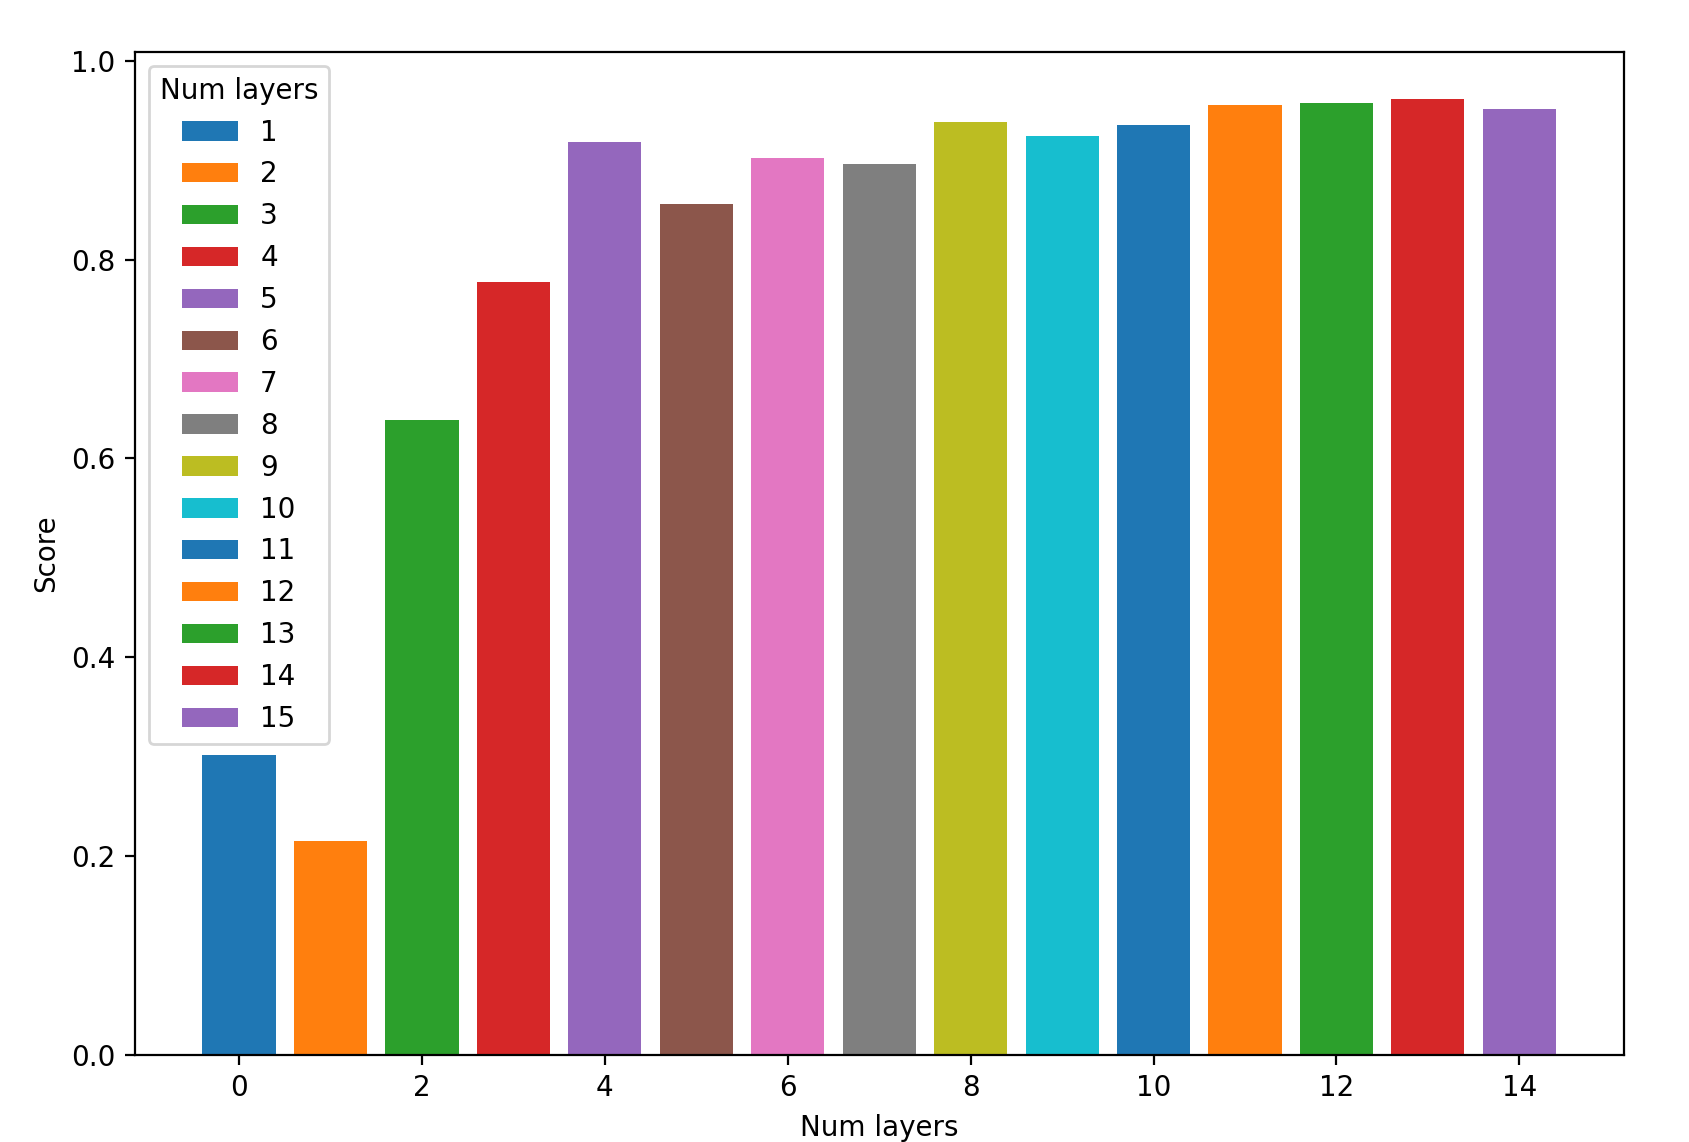
\includegraphics[scale=0.35]{Figure_1}
        %\end{center}

        Here I can see that afther 8 nodes there is litle change in the score.

        \paragraph{Numer of hidden layers}
        Afther testing how many nodes in 1 layer looks good. I proseeded to test how many hidden layers I can use with 8 nodes in. For this I uesd the \texttt{plotMulti3()}

        %\begin{center}
        %    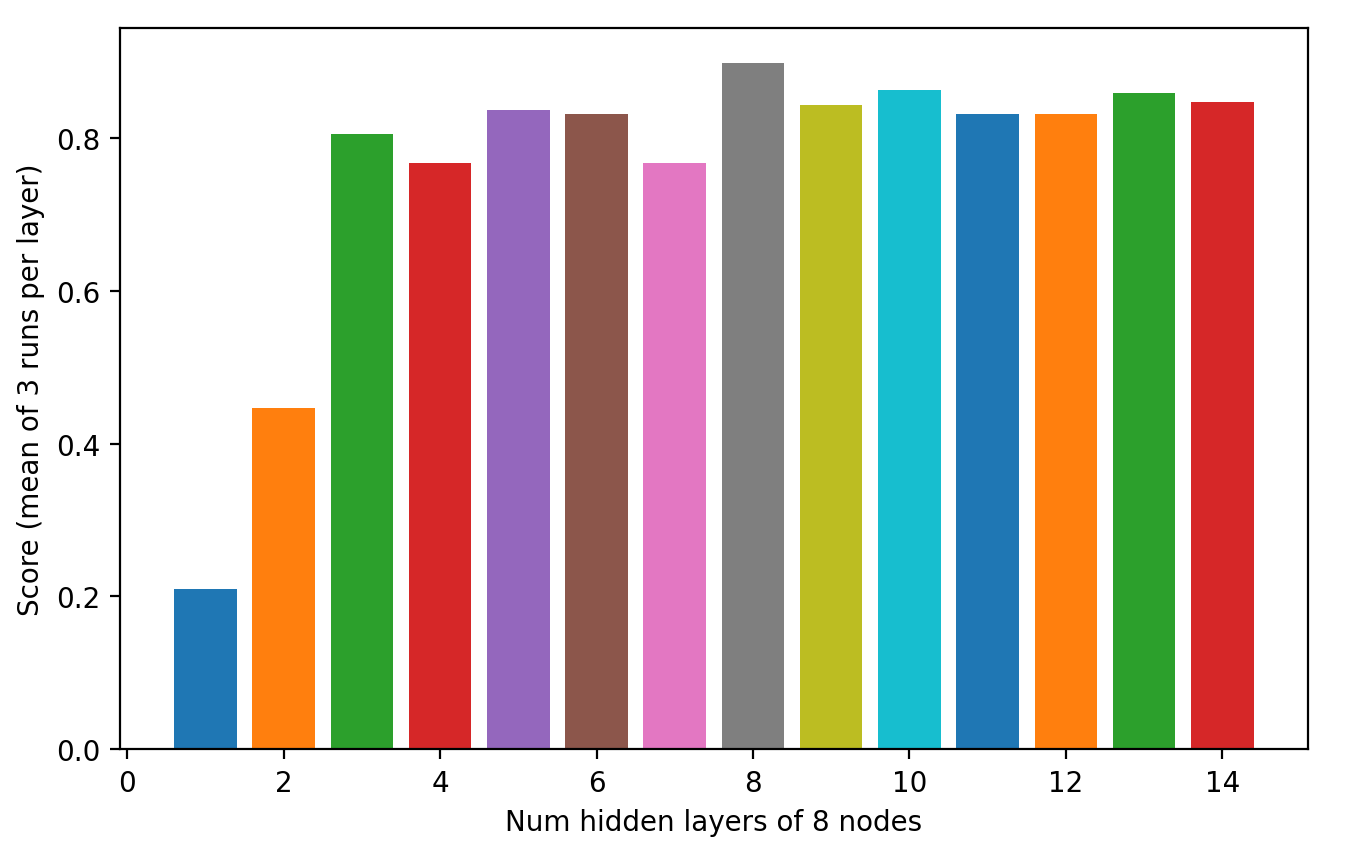
\includegraphics[scale=0.45]{Figure_2}
        %\end{center}

        

        \paragraph{Accuracy}

\end{document}